\documentclass[11pt]{standalone}
% TikZ
    \usepackage{tikz, pgfornament, tikzrput}
    \usetikzlibrary{decorations, decorations.text}
% font size
    \usepackage{fix-cm}
% cryillic font
    \usepackage[OT1]{fontenc}
   
    
    
\begin{document}
    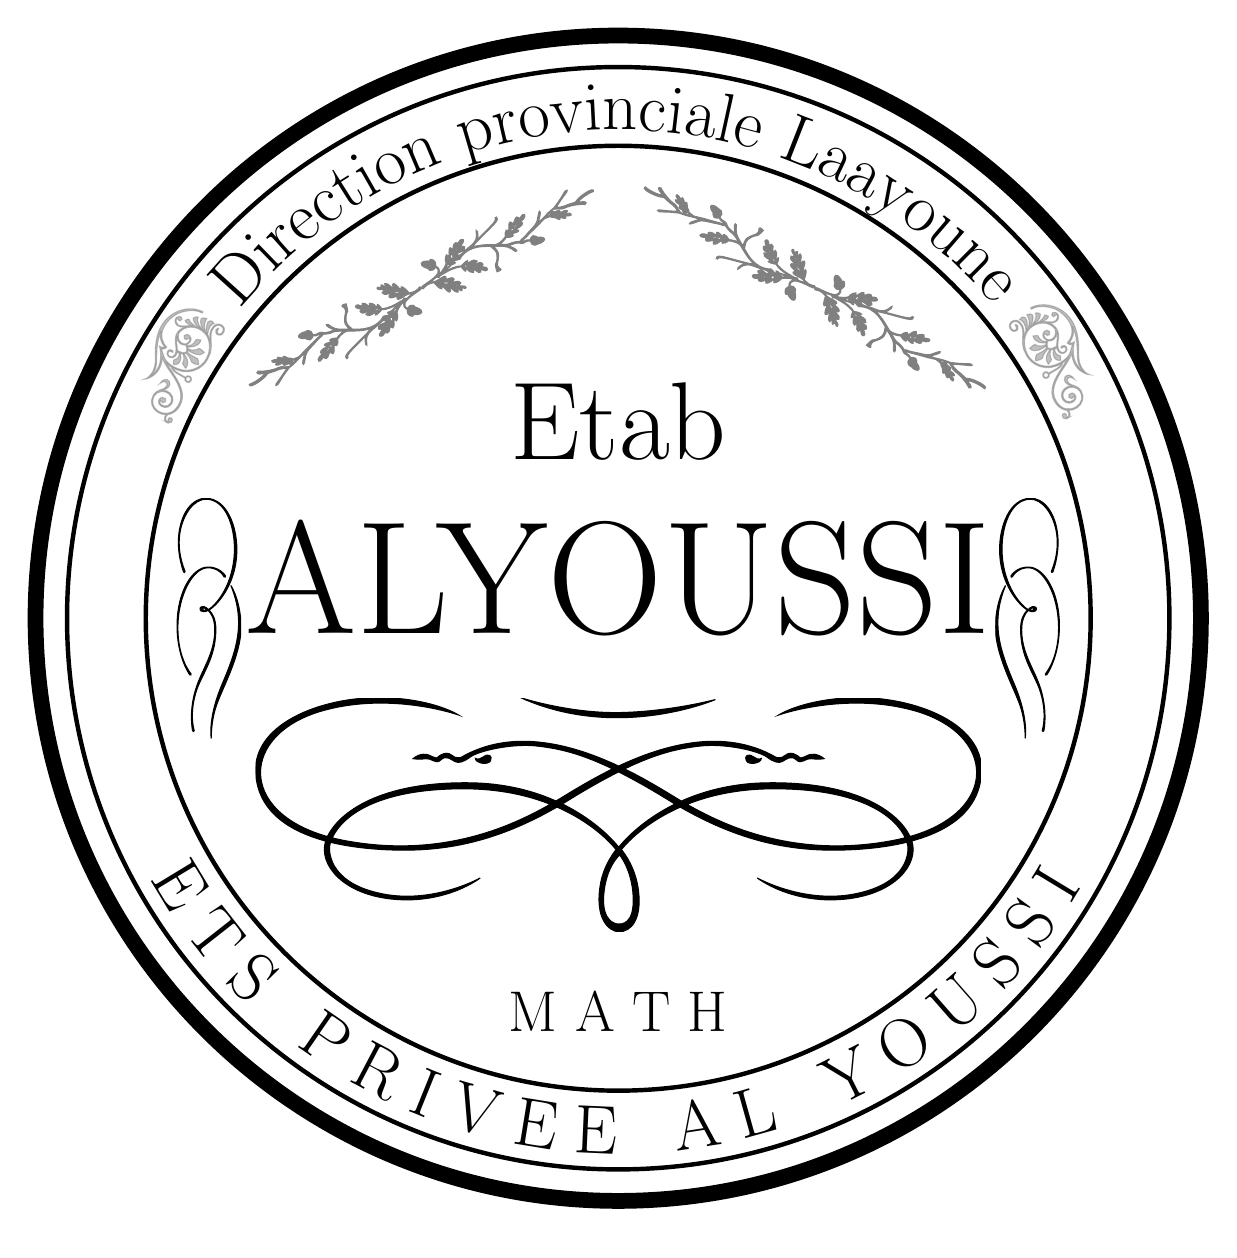
\begin{tikzpicture}
        % outer circle
            \draw[line width=2 mm] circle[radius=7.4 cm];
        % inner circles
            \draw[ultra thick] circle[radius=6 cm] circle[radius=7 cm]  ;
        % outer text
            \path[
                %rotate=-15.2,
                postaction={
                    decoration={
                        text along path,
                        text format delimiters={|}{|},
                        text={%
                            |\Huge|                            
                            {\pgfornament[scale=.4,opacity=0.5, color=gray,ydelta=-9 pt]{15}}
                           Direction provinciale Laayoune
                            {\pgfornament[scale=.4,opacity=0.5, color=gray,ydelta=-9 pt]{16}}
                        },
                        text align=center,
                        reverse path
                    },
                    decorate
                }
            ]
             (-27:6.2cm) arc (-27:210:6.2cm);   
\path [postaction={decorate,decoration={text along path, text align=fit to path,text={|\Huge|ETS PRIVEE AL YOUSSI}}}] (209:6.8cm) arc (209:330:6.8cm);
        % top ornamentation
            \rput{-30}(2.5, 4.2){\pgfornament[scale=.4,opacity=1,color=gray]{87}}
            \rput{30}(-2.5, 4.2){\pgfornament[scale=.4,opacity=1,color=gray]{87}}
        % bottom ornamentation
            \rput(0, -2.5){\pgfornament[scale=.7]{75}}
        % right ornamentation
            \rput{-90}(5.2, 0){\pgfornament[scale=.4]{72}}
        % left ornamentation
            \rput{90}(-5.2, 0){\pgfornament[scale=.4, symmetry=v]{72}}
        % central text
            \node[font=\fontsize{40}{60}\selectfont] at (0, 2.5){Etab};
            \node[font=\fontsize{58}{58}\selectfont] at (0, 0.5){{ALYOUSSI}};
            \node[font=\huge] at (0, -5){ M A T H};
    \end{tikzpicture}
    
    
    \end{document}